%%%%%%%%%%%%%%%%%%%%%%%%%%%%%%%%%%%%%%%%%
% Beamer Presentation
% LaTeX Template
% Version 1.0 (10/11/12)
%
% This template has been downloaded from:
% http://www.LaTeXTemplates.com
%
% License:
% CC BY-NC-SA 3.0 (http://creativecommons.org/licenses/by-nc-sa/3.0/)
%
%%%%%%%%%%%%%%%%%%%%%%%%%%%%%%%%%%%%%%%%%

%----------------------------------------------------------------------------------------
%	PACKAGES AND THEMES
%----------------------------------------------------------------------------------------

\documentclass{beamer}


\mode<presentation> {

% The Beamer class comes with a number of default slide themes
% which change the colors and layouts of slides. Below this is a list
% of all the themes, uncomment each in turn to see what they look like.

%\usetheme{default}
%\usetheme{AnnArbor}
%\usetheme{Antibes}
%\usetheme{Bergen}
%\usetheme{Berkeley}
%\usetheme{Berlin}
%\usetheme{Boadilla}
%\usetheme{CambridgeUS}
%\usetheme{Copenhagen}
%\usetheme{Darmstadt}
%\usetheme{Dresden}
\usetheme{Frankfurt}
%\usetheme{Goettingen}
%\usetheme{Hannover}
%\usetheme{Ilmenau}
%\usetheme{JuanLesPins}
%\usetheme{Luebeck}
%\usetheme{Madrid}
%\usetheme{Malmoe}
%\usetheme{Marburg}
%\usetheme{Montpellier}
%\usetheme{PaloAlto}
%\usetheme{Pittsburgh}
%\usetheme{Rochester}
%\usetheme{Singapore}
%\usetheme{Szeged}
%\usetheme{Warsaw}

% As well as themes, the Beamer class has a number of color themes
% for any slide theme. Uncomment each of these in turn to see how it
% changes the colors of your current slide theme.

%\usecolortheme{albatross}
\usecolortheme{beaver}
%\usecolortheme{beetle}
%\usecolortheme{crane}
%\usecolortheme{dolphin}
%\usecolortheme{dove}
%\usecolortheme{fly}
%\usecolortheme{lily}
%\usecolortheme{orchid}
%\usecolortheme{rose}
%\usecolortheme{seagull}
%\usecolortheme{seahorse}
%\usecolortheme{whale}
%\usecolortheme{wolverine}

%\setbeamertemplate{footline} % To remove the footer line in all slides uncomment this line
\setbeamertemplate{footline}[page number] % To replace the footer line in all slides with a simple slide count uncomment this line

\setbeamercolor*{item}{fg=red!60!black}

\useinnertheme{rectangles}

%\setbeamertemplate{navigation symbols}{} % To remove the navigation symbols from the bottom of all slides uncomment this line
}

\usepackage{graphicx} % Allows including images
\usepackage{booktabs} % Allows the use of \toprule, \midrule and \bottomrule in tables
\usepackage{epstopdf}

%----------------------------------------------------------------------------------------
%	TITLE PAGE
%----------------------------------------------------------------------------------------

\title[Short title]{\textbf{WebRTC on Mobile Edge Cloud}} % The short title appears at the bottom of every slide, the full title is only on the title page

\author{\textbf{Dr. Ahmad Al-Shishtawy, Qi Qi}} % Your name
\institute[SICS Swedish ICT] % Your institution as it will appear on the bottom of every slide, may be shorthand to save space
{
Swedish Institute of Computer Science \\ \textit{SICS Swedish ICT}\\ % Your institution for the title page
\medskip
\textit{ahmad@sics.se, qiq@sics.se} % Your email address
}
\date{4 December, 2014} % Date, can be changed to a custom date

\logo{
\includegraphics[scale=0.1]{figs/sics.eps}}

\begin{document}

\begin{frame}
\titlepage % Print the title page as the first slide
\end{frame}

%\begin{frame}
%\frametitle{Overview} % Table of contents slide, comment this block out to remove it
%\tableofcontents % Throughout your presentation, if you choose to use \section{} and \subsection{} commands, these will automatically be printed on this slide as an overview of your presentation
%\end{frame}

%----------------------------------------------------------------------------------------
%	PRESENTATION SLIDES
%----------------------------------------------------------------------------------------

%------------------------------------------------
\section{Introduction} 
%------------------------------------------------
\subsection{Motivation}
\begin{frame}
\frametitle{Motivation}
\begin{alertblock}{WebRTC}
\begin{enumerate}
	\item Open source plugin-free real-time communication in browsers
	\item More than 1 billion unique cross platform endpoints 
	\item Peer-to-peer optimization as a service required
\end{enumerate}
\end{alertblock}

\begin{alertblock}{Mobile Edge Cloud}
\begin{enumerate}
	\item Deployed on access network layer
	\item Low latency to mobile end-users
	\item "Smart proxy" to process media stream prior to the forwarding
\end{enumerate}
\end{alertblock}
\end{frame}
%------------------------------------------------
\subsection{Concept}
\begin{frame}
\frametitle{Concept}
\begin{figure}[h!]
	\centering
	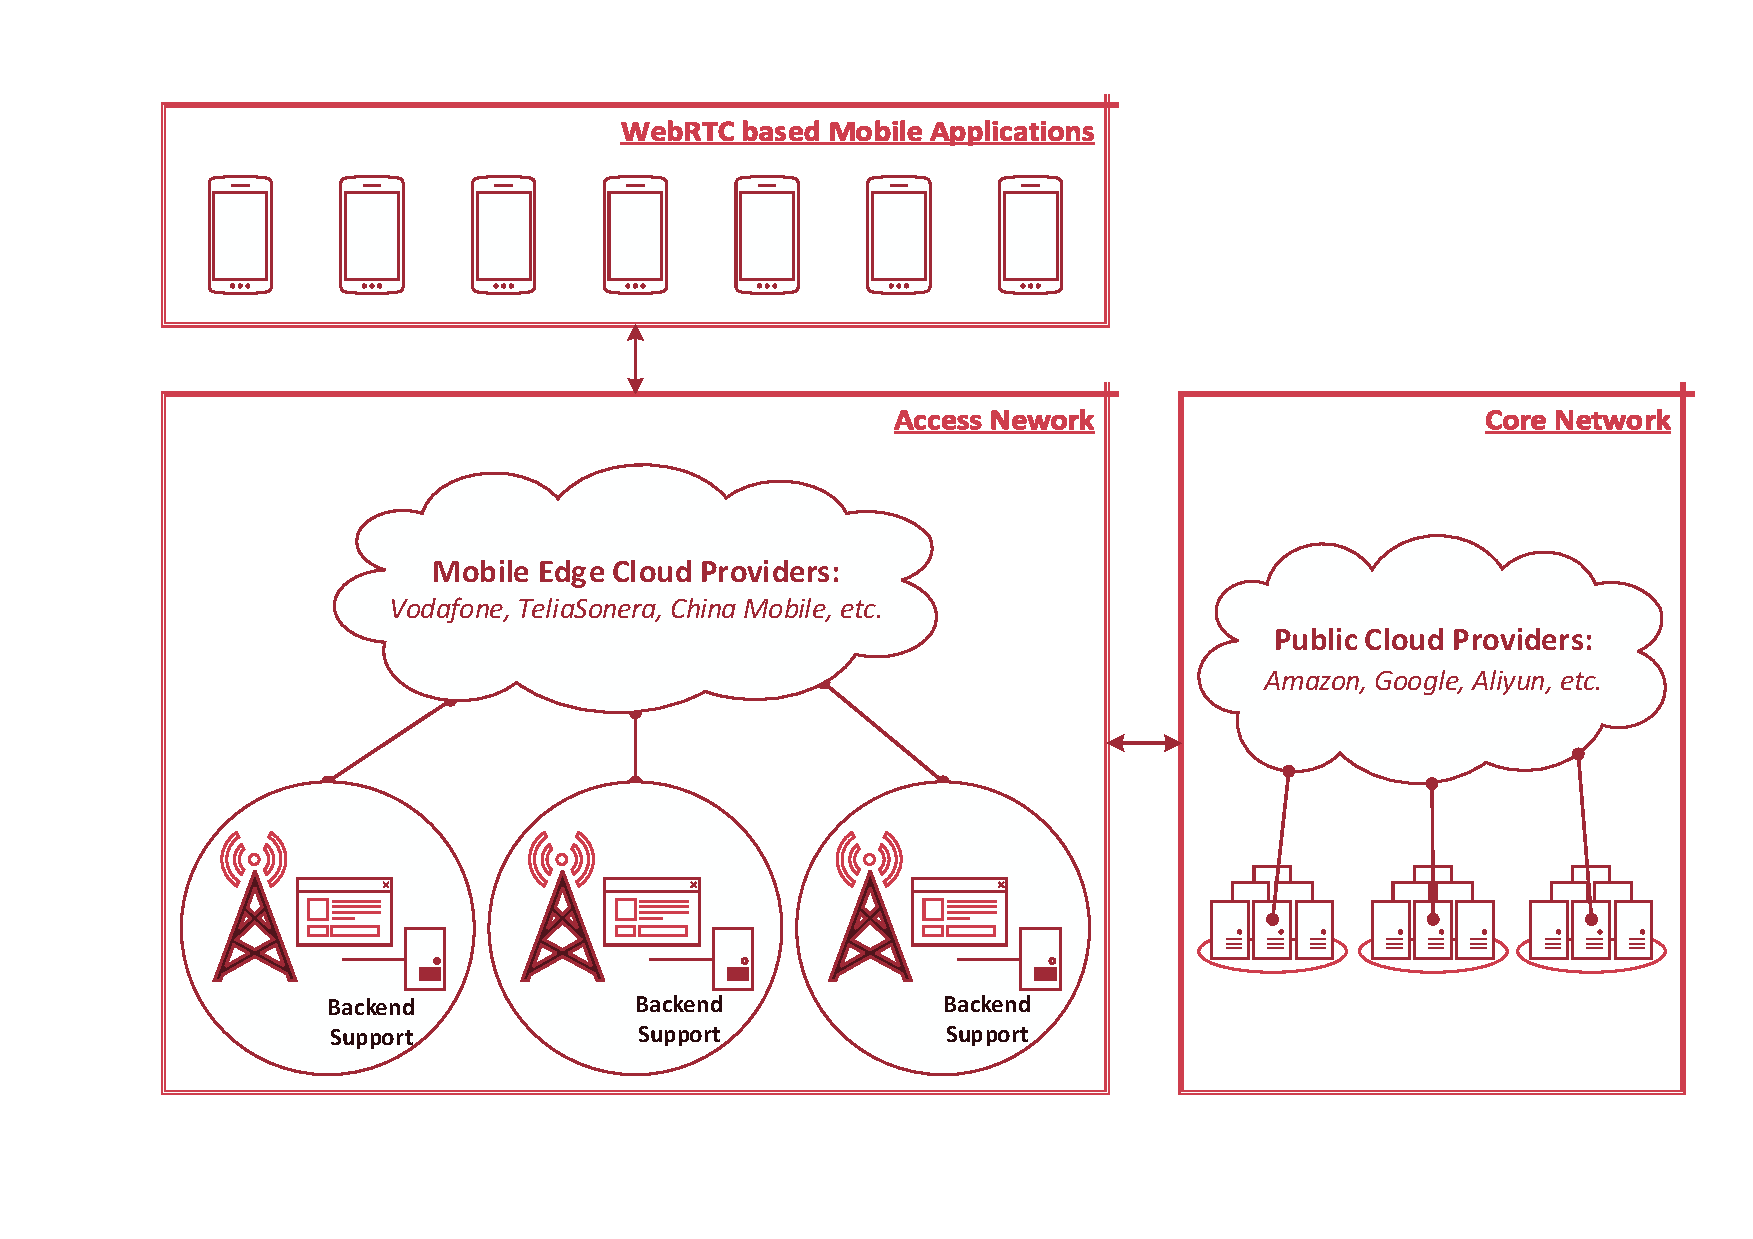
\includegraphics[scale=0.4]{figs/concept.pdf}
\end{figure}
\end{frame}
%------------------------------------------------
\subsection{Summary}
\begin{frame}
\frametitle{Summary}
\begin{alertblock}{Exchange}
real-time video, audio and data between browsers
\end{alertblock}

\begin{alertblock}{Deploy}
backend services on mobile edge cloud
\end{alertblock}

\begin{alertblock}{Improve}
user experience on WebRTC based mobile applications
\end{alertblock}

\begin{alertblock}{Reduce}
bandwidth consumption for mobile network operators
\end{alertblock}
\end{frame}

%------------------------------------------------
\section{Signaling Service}
%------------------------------------------------
\subsection{Signaling Service (1/2)}
\begin{frame}
	\frametitle{Signaling Service (1/2)}
	\begin{enumerate}
		\item Initiate a peer-to-peer connection
		\item Exchange session description
		\item Not specified by WebRTC
	\end{enumerate}
\end{frame}

\subsection{Signaling Service (2/2)}
\begin{frame}
	\frametitle{Signaling Service (2/2)}
	\begin{figure}[h!]
		\centering
		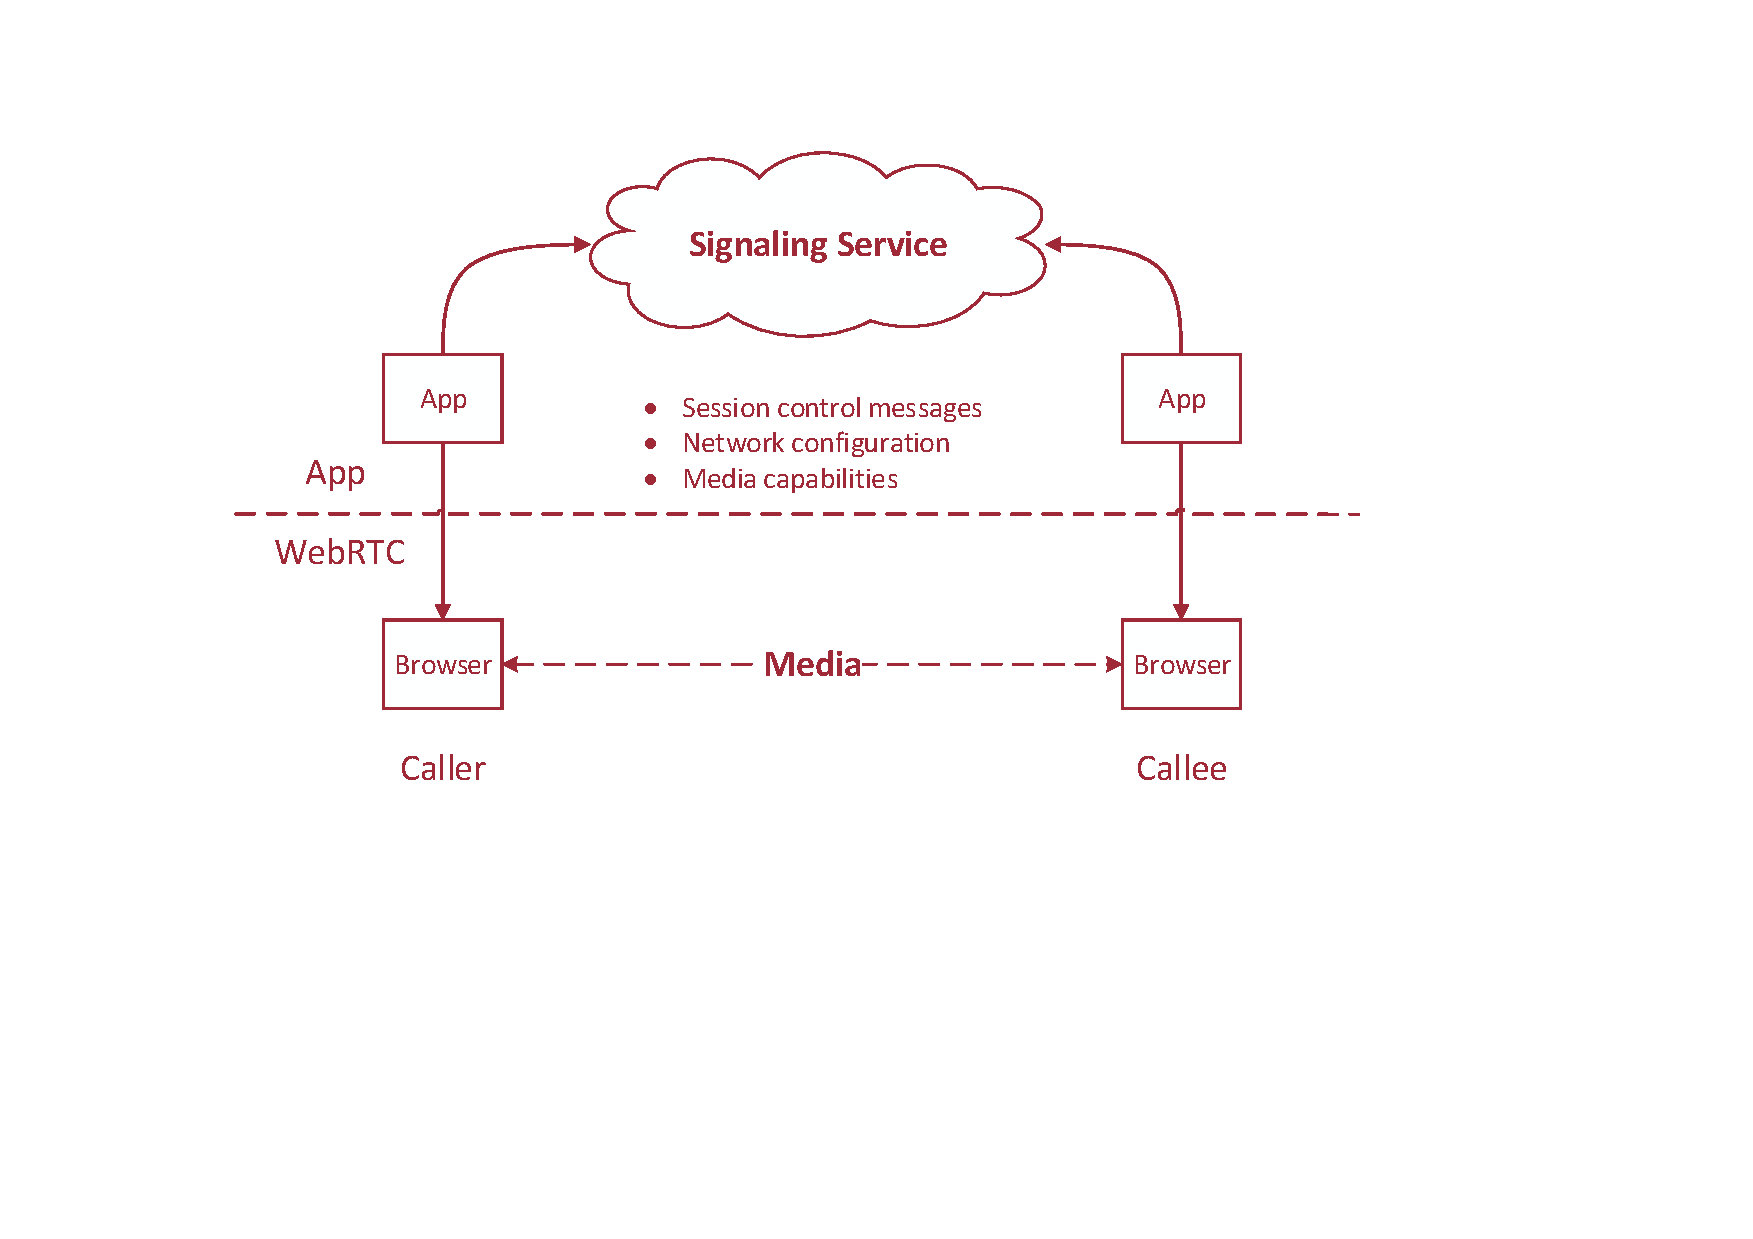
\includegraphics[scale=0.6]{figs/signal.pdf}
	\end{figure}
\end{frame}

%------------------------------------------------
\section{Firewall and NAT Traversal}
%------------------------------------------------
\subsection{Firewall and NAT Traversal (1/2)}
\begin{frame}
\frametitle{Firewall and NAT Traversal (1/2)}
	\begin{enumerate}
		\item STUN: Session Traversal Utilities for NAT
		\item TURN: Traversal Using Relays around NAT
		\item ICE: Interactive Connectivity Establishment
	\end{enumerate}
\end{frame}

\subsection{Firewall and NAT Traversal (2/2)}
\begin{frame}
	\frametitle{Firewall and NAT Traversal (2/2)}
		\begin{figure}[h!]
			\centering
			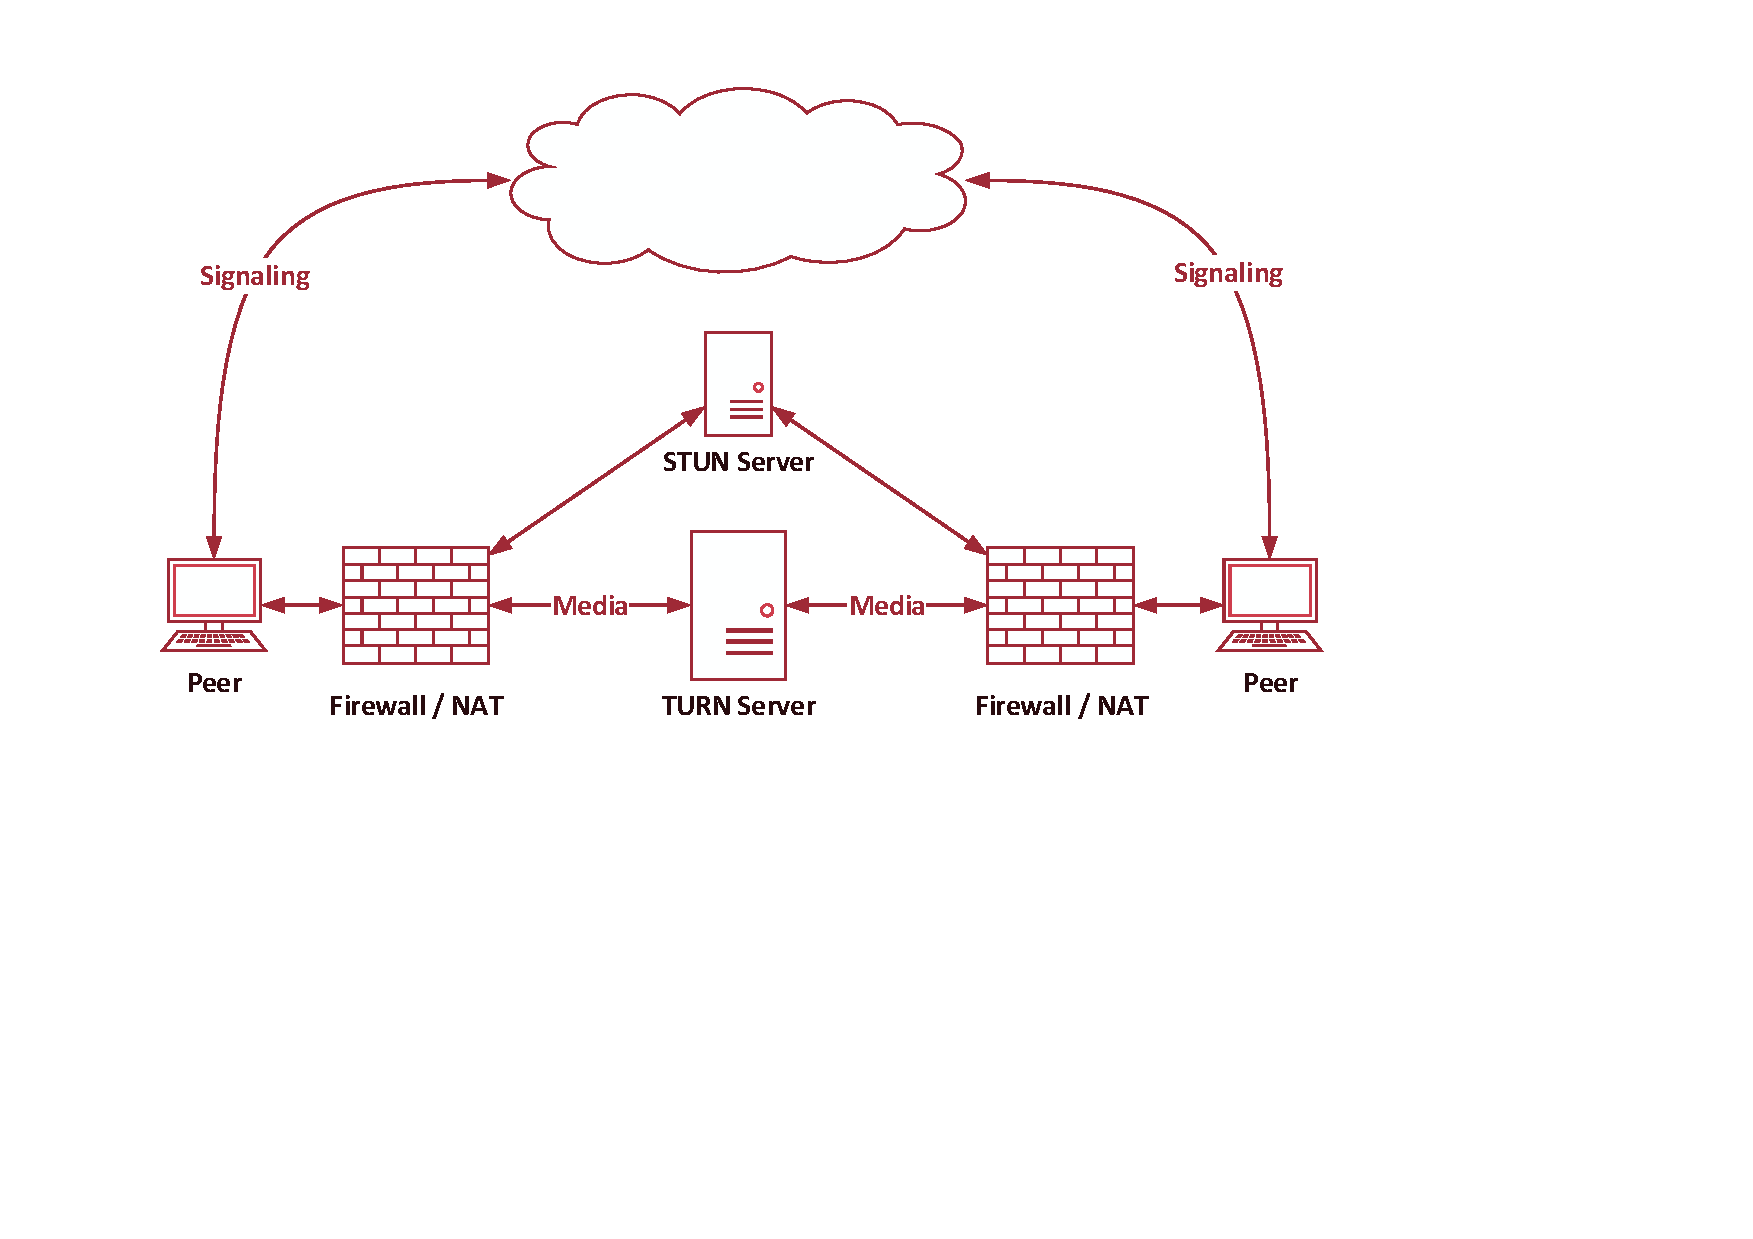
\includegraphics[scale=0.55]{figs/nat.pdf}
		\end{figure}
\end{frame}
%------------------------------------------------
\section{Multiparty Communication}
%------------------------------------------------
\subsection{Mesh Network}
\begin{frame}
\frametitle{Mesh Network}
Simple but inefficient.
		\begin{figure}[h!]
			\centering
			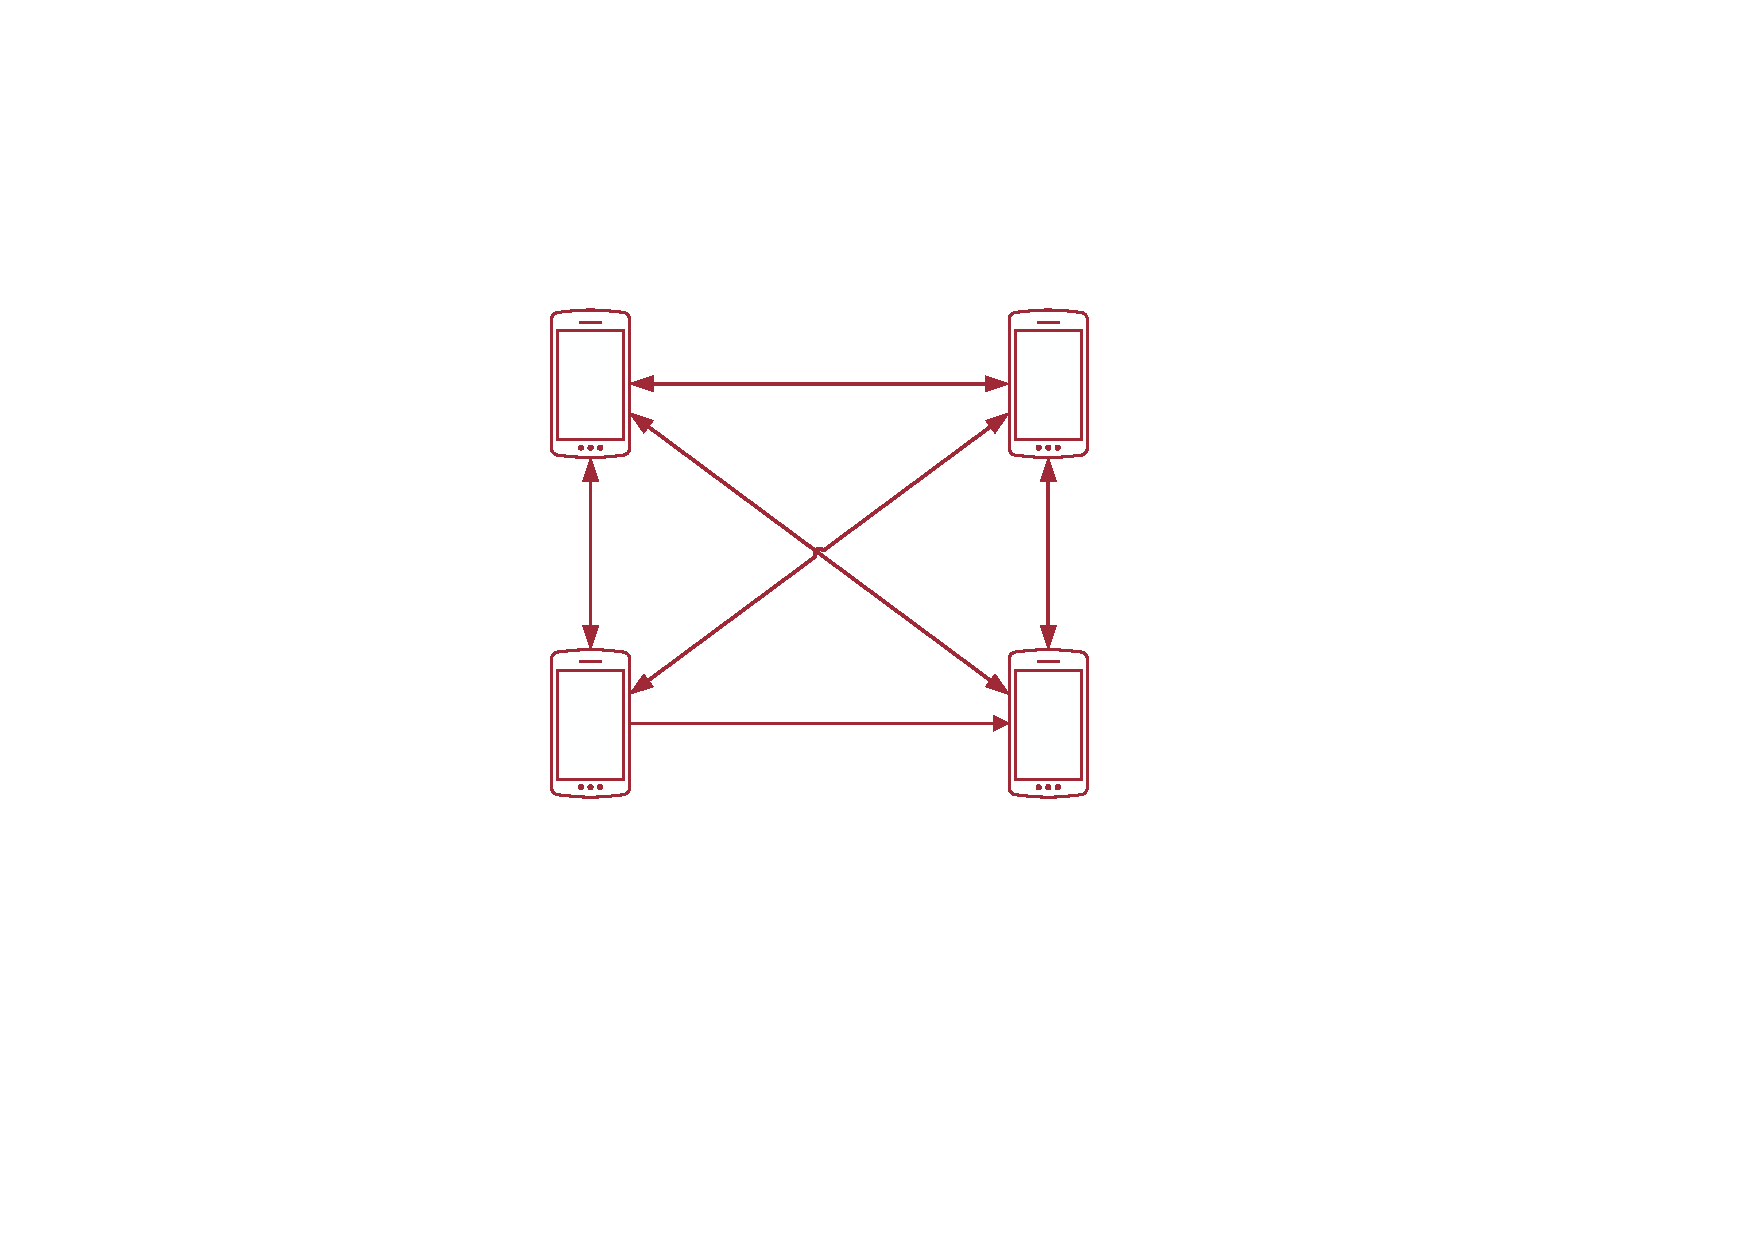
\includegraphics[scale=0.6]{figs/mesh.pdf}
		\end{figure}
\end{frame}
%------------------------------------------------
\subsection{Star Network}
\begin{frame}
	\frametitle{Star Network}
	Too much traffic on single peer.
	\begin{figure}[h!]
		\centering
		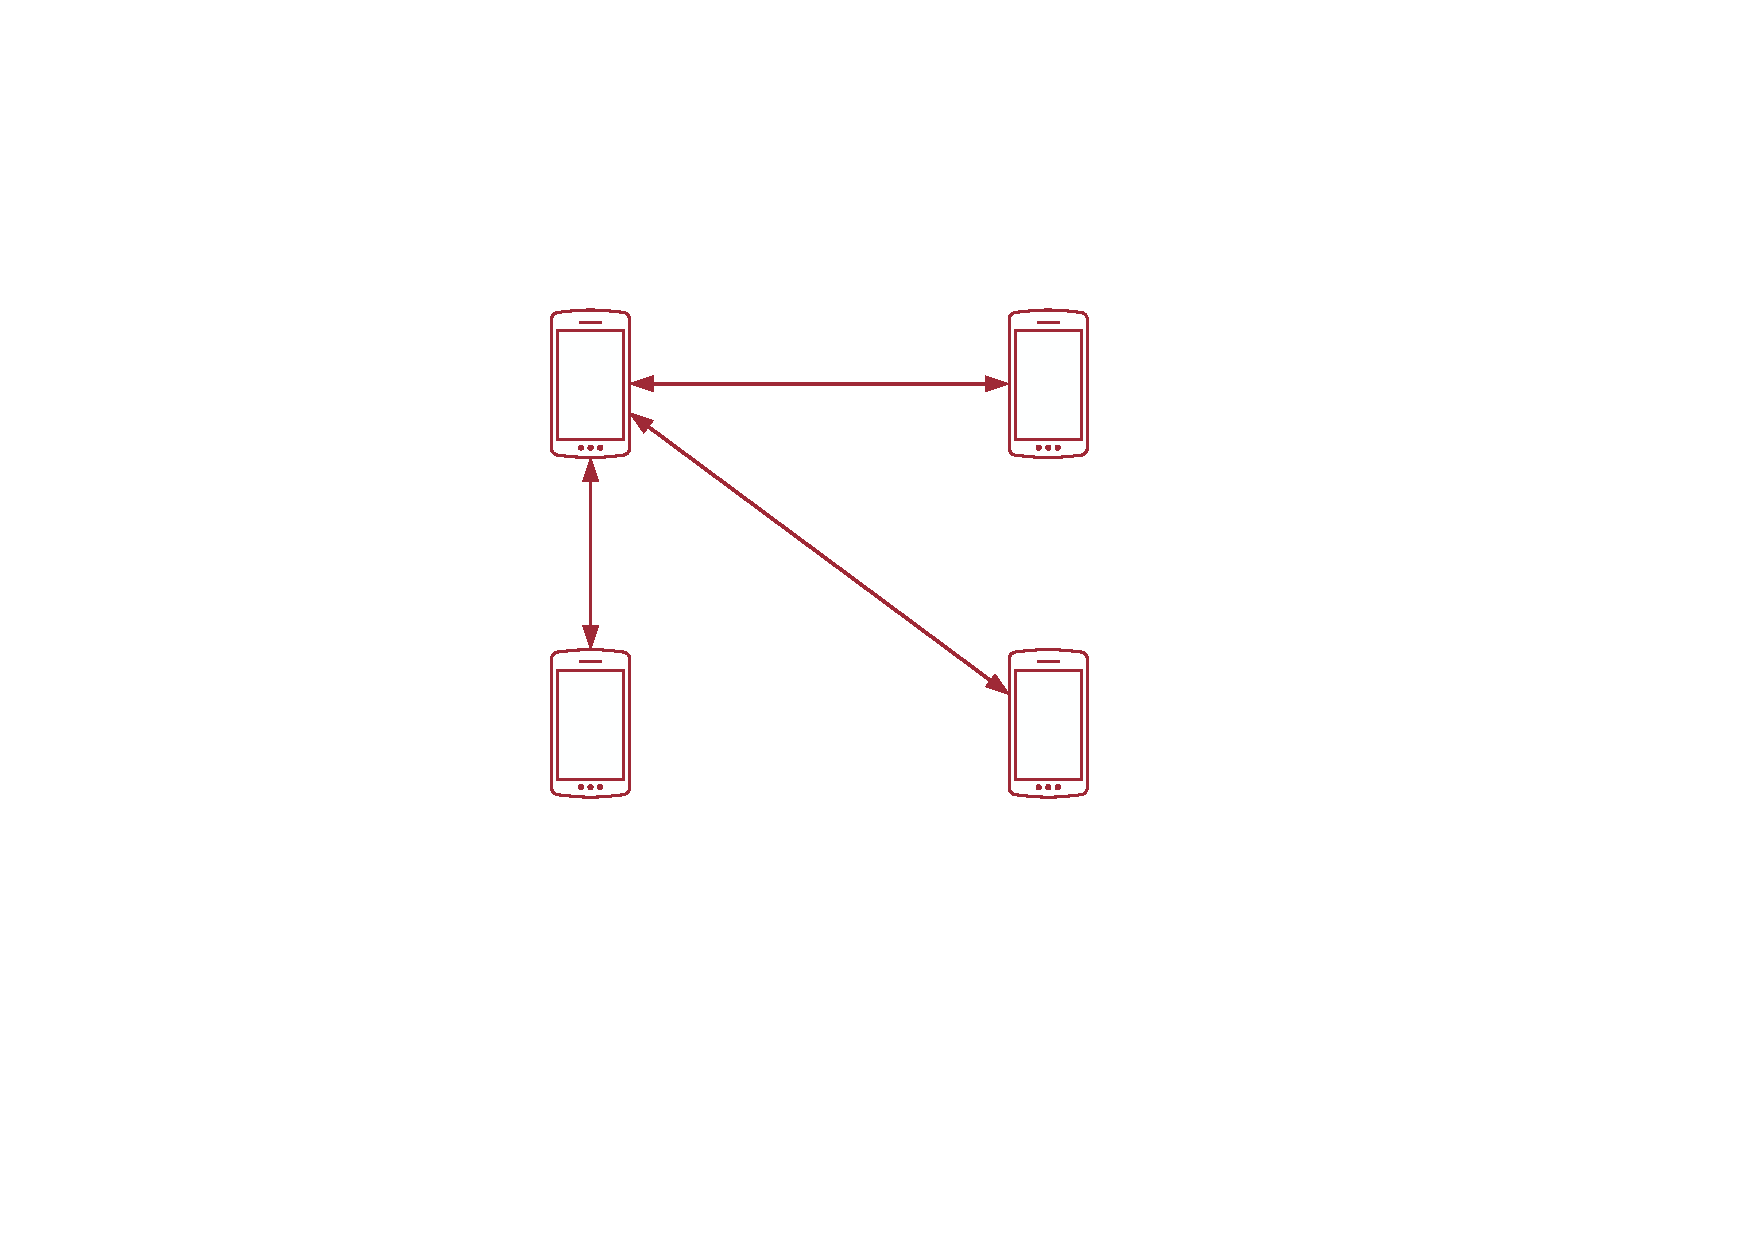
\includegraphics[scale=0.6]{figs/star.pdf}
	\end{figure}
\end{frame}
%------------------------------------------------
\subsection{Mixer Solution}
\begin{frame}
	\frametitle{Mixer Solution}
	Multipoint Control Unit (MCU) - a central point transcodes stream and maintains a single one-to-one stream with each peer
	\begin{figure}[h!]
		\centering
		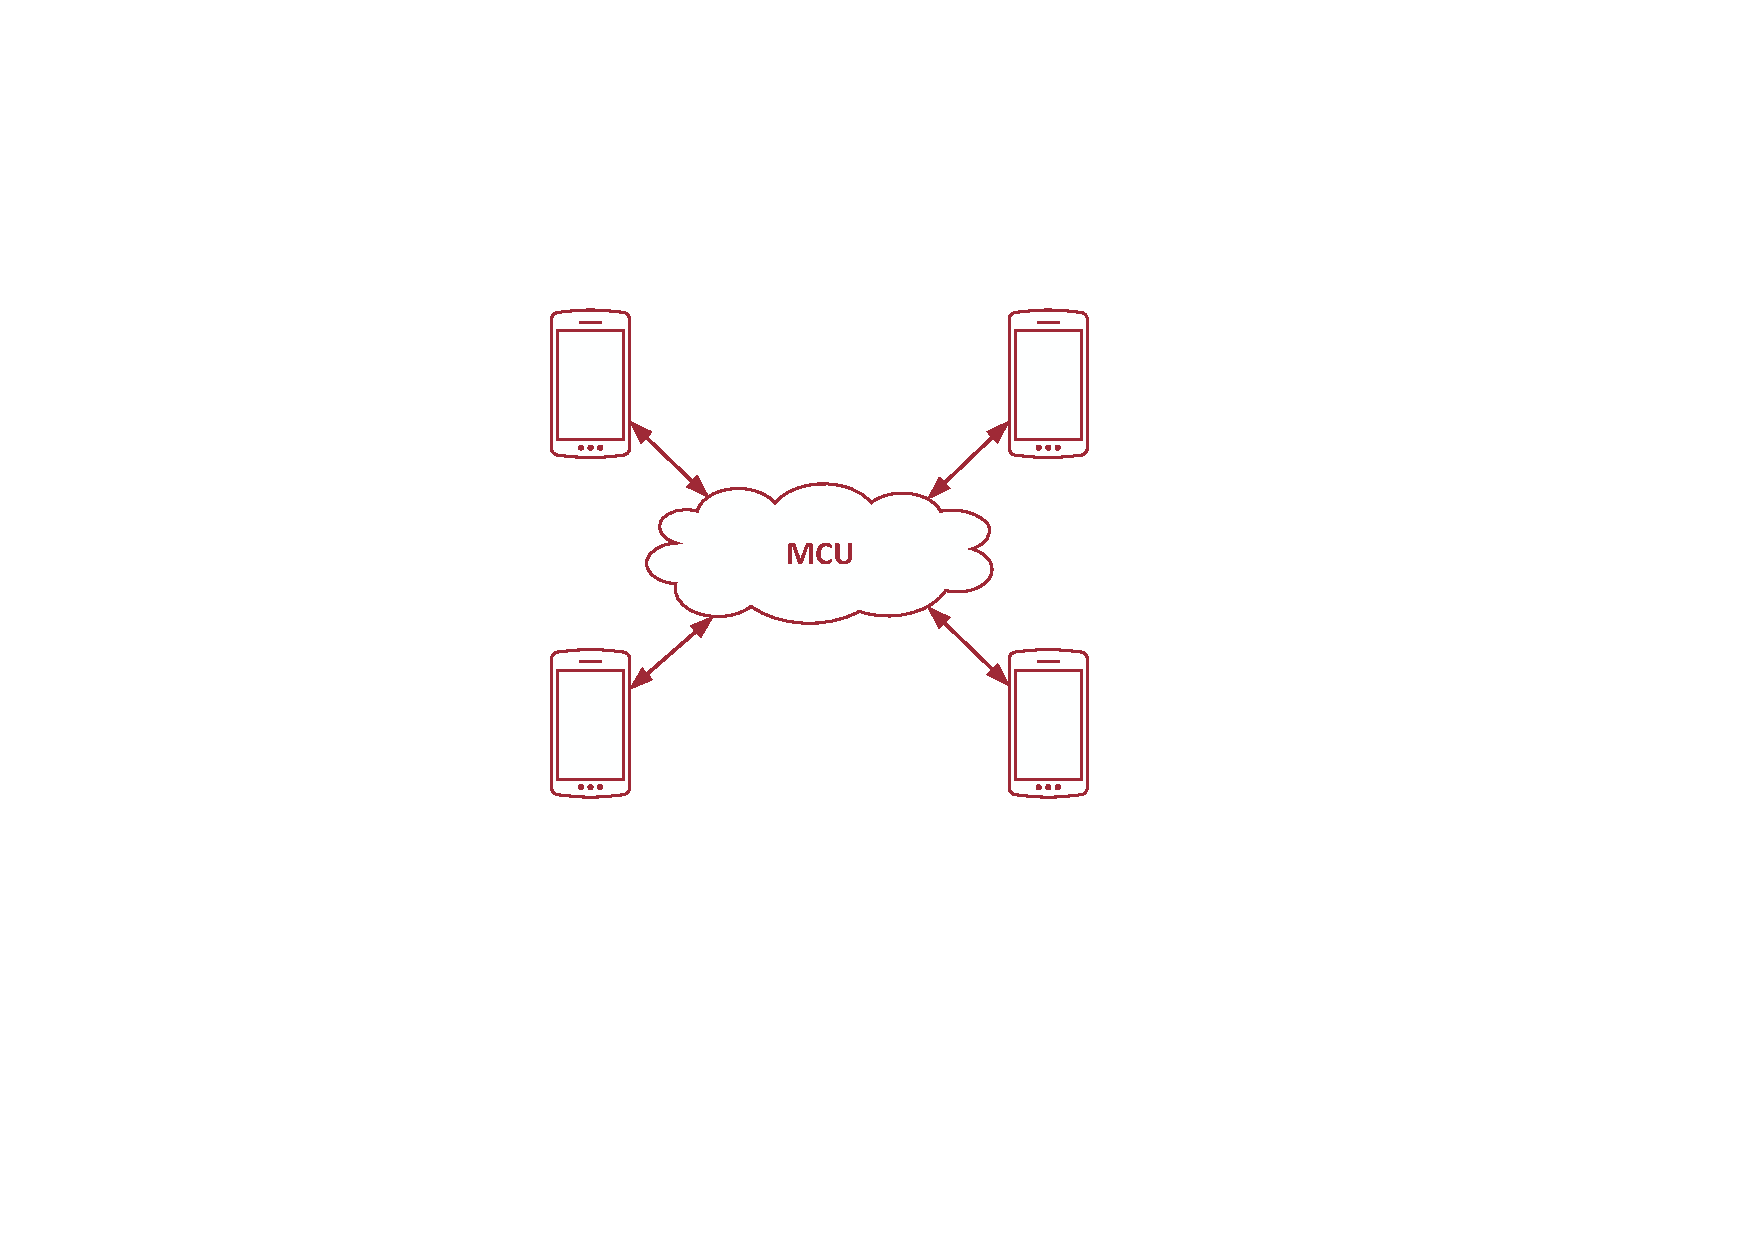
\includegraphics[scale=0.6]{figs/mcu.pdf}
	\end{figure}
\end{frame}
%------------------------------------------------
\subsection{Router Solution}
\begin{frame}
	\frametitle{Router Solution}
	 Relay approach - a central point inspects and forwards stream 
	\begin{figure}[h!]
		\centering
		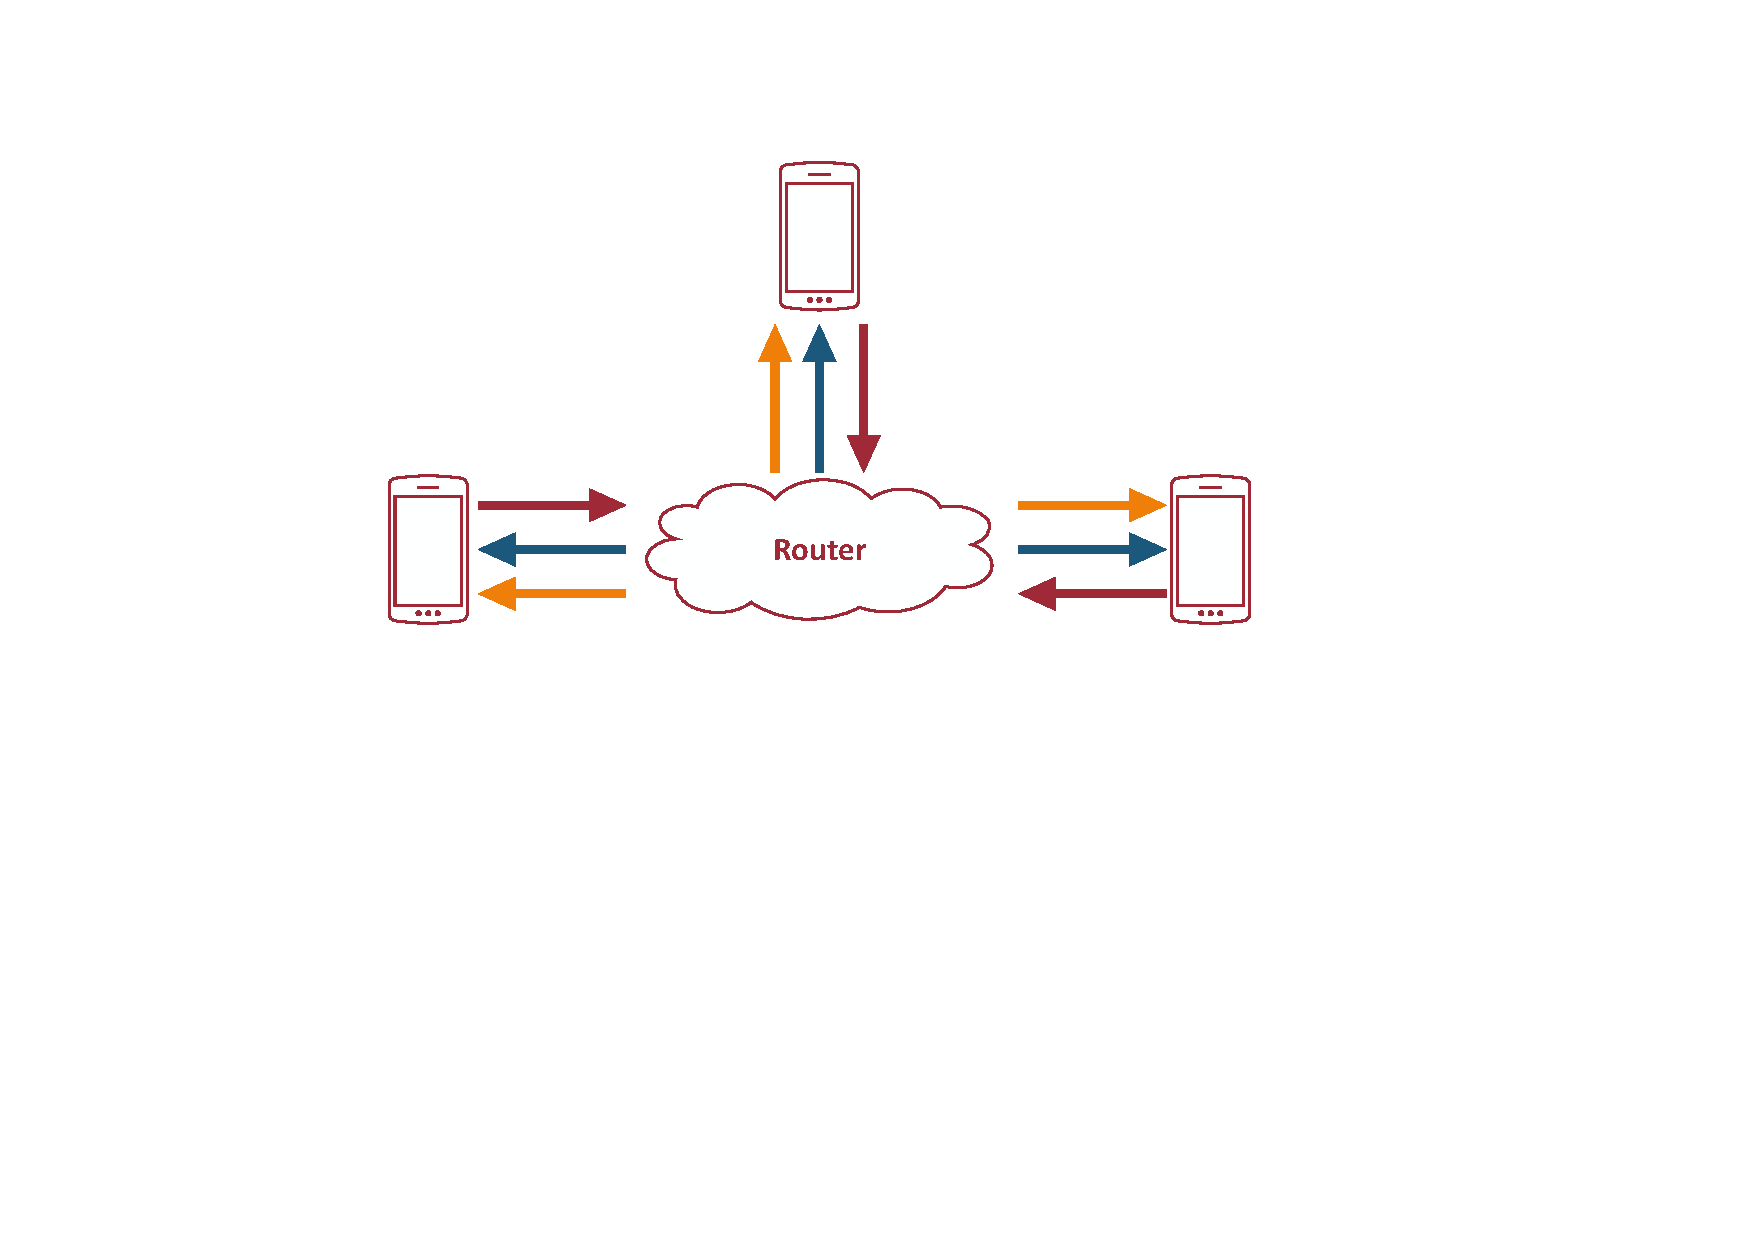
\includegraphics[scale=0.6]{figs/router.pdf}
	\end{figure}
\end{frame}
%------------------------------------------------
\section{Demo}
%------------------------------------------------
\subsection{Demo}
\begin{frame}
\frametitle{Demo}
\Huge{\centerline{Demo}}
\end{frame}
\begin{frame}
\frametitle{The End}
\Huge{\centerline{Thank you!}}
\end{frame}

%----------------------------------------------------------------------------------------

\end{document} 